\documentclass[article, 1.5space, letterpaper, 12pt, oneside, header, footer]{SydeClass}
\graphicspath{{images/}}
\usepackage{subfigure}
\usepackage{eqnarray}


% --------- Title Info -----------
\titlestyle{design} % used in SydeTitle.tex. Can equal one of the following values: design, work

\title{Lab 1}
\subtitle{Fundamentals of Image Processing}

\coursecode{SYDE 475}
\department{Systems Design Engineering}

\author{Colin Heics, 20240543}
\authorheader{C. Heics}
\authortwo{Neil Sokol, 20265064}
\authorheadertwo{N. Sokol}

\date{\today}
\instructor{Alex Wong}

\subsectionfont{\normalsize}
\setcounter{secnumdepth}{2}
\setcounter{tocdepth}{1}

\usepackage{listings}
\usepackage{color}
\usepackage{textcomp}
\definecolor{listinggray}{gray}{0.9}
\definecolor{lbcolor}{rgb}{0.9,0.9,0.9}
\lstset{
	backgroundcolor=\color{lbcolor},
	tabsize=4,
	rulecolor=,
	language=matlab,
        basicstyle=\scriptsize,
        upquote=true,
        aboveskip={1.5\baselineskip},
        columns=fixed,
        showstringspaces=false,
        extendedchars=true,
        breaklines=true,
        prebreak = \raisebox{0ex}[0ex][0ex]{\ensuremath{\hookleftarrow}},
        frame=single,
        showtabs=false,
        showspaces=false,
        showstringspaces=false,
        identifierstyle=\ttfamily,
        keywordstyle=\color[rgb]{0,0,1},
        commentstyle=\color[rgb]{0.133,0.545,0.133},
        stringstyle=\color[rgb]{0.627,0.126,0.941},
}

% ############  ############
\begin{document}

% ---------- Title ------------

%% Use the command "
%% Use the command "
%% Use the command "\input{SydeTitle}" in your main file to include this file.

\begin{titlepage}
	\makeatletter % use .cls usage for <at>
	
	\pagestyle{empty}
	\equalmargins
	
	\ifthenelse{\equal{\@titlestyle}{work}}{
		\begin{center}
			\vspace*{2em}

			University of Waterloo\\
			Faculty of Engineering\\
			Department of Systems Design Engineering

			\null\vfill
		
			\Huge\@title \\
			\ifdefined \@subtitle \Large\@subtitle \\ \fi
			\normalsize

			\null\vfill
		
			\@company\\
			\@companyaddress \vspace{2em}
		
			\@author\\
			\@date
		\end{center}
	}{\relax} % end if
	
	\ifthenelse{\equal{\@titlestyle}{design}}{
		\begin{center}
			\vspace*{5em}
	
			\Huge\@title \\
			\ifdefined \@subtitle \Large\@subtitle \\ \fi
			\normalsize
	
			\vfill
		
			A Report Submitted in Partial Fulfilment\\
			of the Requirements for \@coursecode \vspace{4em}
		
			\ifdefined \@groupname \@groupname \\ \fi
		  \@author \\
			\ifdefined \@authortwo \@authortwo \\ \fi
			\ifdefined \@authorthree \@authorthree \\ \fi
			\ifdefined \@authorfour \@authorfour \\ \fi
		  \vspace{3em}
		
			Faculty of Engineering \\
			\ifdefined \@department Department of \@department \\ \fi
			\vspace{3em}
		
			\@date \\
			
			\ifdefined \@instructor Course Instructor: \@instructor \\ \fi
			\ifdefined \@supervisor Project Supervisor: \@supervisor \\ \fi
			
		\end{center}
	}{\relax} % end if
	
	\makeatother % return to document usage for <at>
\end{titlepage}

%\pagestyle{plain}
%\offsetmargins" in your main file to include this file.

\begin{titlepage}
	\makeatletter % use .cls usage for <at>
	
	\pagestyle{empty}
	\equalmargins
	
	\ifthenelse{\equal{\@titlestyle}{work}}{
		\begin{center}
			\vspace*{2em}

			University of Waterloo\\
			Faculty of Engineering\\
			Department of Systems Design Engineering

			\null\vfill
		
			\Huge\@title \\
			\ifdefined \@subtitle \Large\@subtitle \\ \fi
			\normalsize

			\null\vfill
		
			\@company\\
			\@companyaddress \vspace{2em}
		
			\@author\\
			\@date
		\end{center}
	}{\relax} % end if
	
	\ifthenelse{\equal{\@titlestyle}{design}}{
		\begin{center}
			\vspace*{5em}
	
			\Huge\@title \\
			\ifdefined \@subtitle \Large\@subtitle \\ \fi
			\normalsize
	
			\vfill
		
			A Report Submitted in Partial Fulfilment\\
			of the Requirements for \@coursecode \vspace{4em}
		
			\ifdefined \@groupname \@groupname \\ \fi
		  \@author \\
			\ifdefined \@authortwo \@authortwo \\ \fi
			\ifdefined \@authorthree \@authorthree \\ \fi
			\ifdefined \@authorfour \@authorfour \\ \fi
		  \vspace{3em}
		
			Faculty of Engineering \\
			\ifdefined \@department Department of \@department \\ \fi
			\vspace{3em}
		
			\@date \\
			
			\ifdefined \@instructor Course Instructor: \@instructor \\ \fi
			\ifdefined \@supervisor Project Supervisor: \@supervisor \\ \fi
			
		\end{center}
	}{\relax} % end if
	
	\makeatother % return to document usage for <at>
\end{titlepage}

%\pagestyle{plain}
%\offsetmargins" in your main file to include this file.

\begin{titlepage}
	\makeatletter % use .cls usage for <at>
	
	\pagestyle{empty}
	\equalmargins
	
	\ifthenelse{\equal{\@titlestyle}{work}}{
		\begin{center}
			\vspace*{2em}

			University of Waterloo\\
			Faculty of Engineering\\
			Department of Systems Design Engineering

			\null\vfill
		
			\Huge\@title \\
			\ifdefined \@subtitle \Large\@subtitle \\ \fi
			\normalsize

			\null\vfill
		
			\@company\\
			\@companyaddress \vspace{2em}
		
			\@author\\
			\@date
		\end{center}
	}{\relax} % end if
	
	\ifthenelse{\equal{\@titlestyle}{design}}{
		\begin{center}
			\vspace*{5em}
	
			\Huge\@title \\
			\ifdefined \@subtitle \Large\@subtitle \\ \fi
			\normalsize
	
			\vfill
		
			A Report Submitted in Partial Fulfilment\\
			of the Requirements for \@coursecode \vspace{4em}
		
			\ifdefined \@groupname \@groupname \\ \fi
		  \@author \\
			\ifdefined \@authortwo \@authortwo \\ \fi
			\ifdefined \@authorthree \@authorthree \\ \fi
			\ifdefined \@authorfour \@authorfour \\ \fi
		  \vspace{3em}
		
			Faculty of Engineering \\
			\ifdefined \@department Department of \@department \\ \fi
			\vspace{3em}
		
			\@date \\
			
			\ifdefined \@instructor Course Instructor: \@instructor \\ \fi
			\ifdefined \@supervisor Project Supervisor: \@supervisor \\ \fi
			
		\end{center}
	}{\relax} % end if
	
	\makeatother % return to document usage for <at>
\end{titlepage}

%\pagestyle{plain}
%\offsetmargins

% ############ Chapters ############
\pagenumbering{arabic}

\section{Introduction}



\section{Image quality measures}

During the lab, some operations will be applied to a modified image in order to improve it's appearance. In order to evaluate the quality of the operation, a measure known as the ``Peak Signal to Noise Ratio'' (PSNR) is used, calculated as illustrated in \eqref{eqn-psnr}.

\begin{eqnarray}
\label{eqn-psnr}
PSNR & = & 10 \log_{10}\left ( \frac{{\textup{MAX}_f}^{2}}{\textup{MSE}} \right ) \\
\textup{MSE} & = &\frac{1}{mn} \sum_{i=0}^{m-1}\sum_{j=0}^{n-1} \left \| f(i,j) - g(i,j) \right \|^2
\end{eqnarray}

The Matlab code used to calculate the PSNR for this lab is attached in Appendix~\ref{code-PSNR}.


\section{Digital zooming}

Digital zooming techniques can introduce artifacts into an image. In order to evaluate several digital zooming techniques, two different sample images will be down scaled by a factor of 4, then enlarged using one of three digital zooming techniques. The resulting images will be compared to the ground truth using PSNR, and are included in Figures~\ref{fig:digitalZoom.lena}~and~\ref{fig:digitalZoom.cameraman}.


\begin{figure}[ht]
\centering
	\subfigure[Original image, PSNR $= \infty$]{
	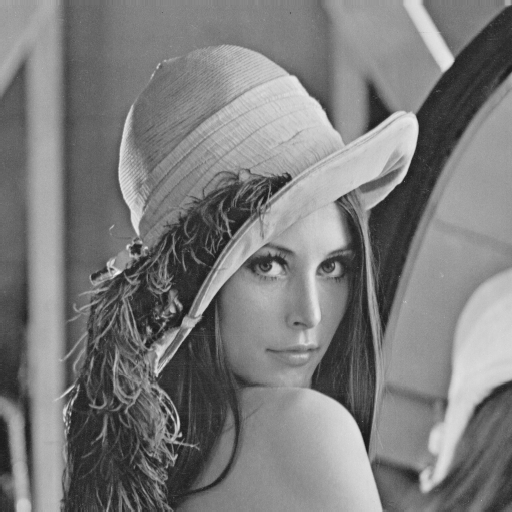
\includegraphics[width=0.45\linewidth]{digitalZoom/lenaBase}
	}
	\subfigure[Nearest Neighbour, PSNR = +33.96 dB]{
	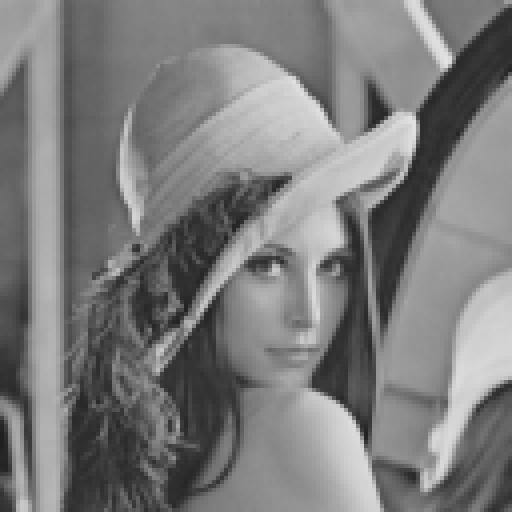
\includegraphics[width=0.45\linewidth]{digitalZoom/lena_NN}
	}
	\subfigure[Bilinear Interpolation, PSNR = +34.26 dB]{
	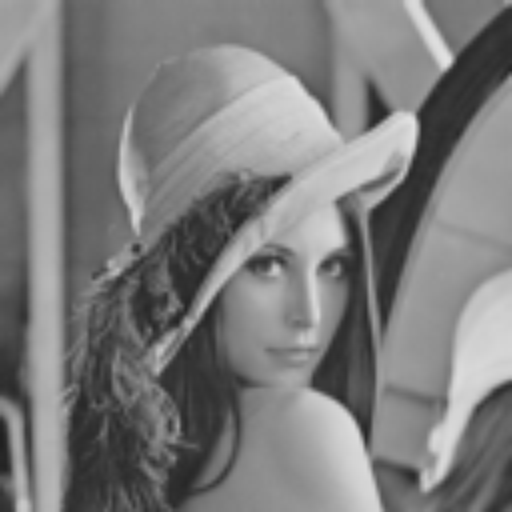
\includegraphics[width=0.45\linewidth]{digitalZoom/lena_BL}
	}
	\subfigure[Bicubic Interpolation, PSNR = +34.70 dB]{
	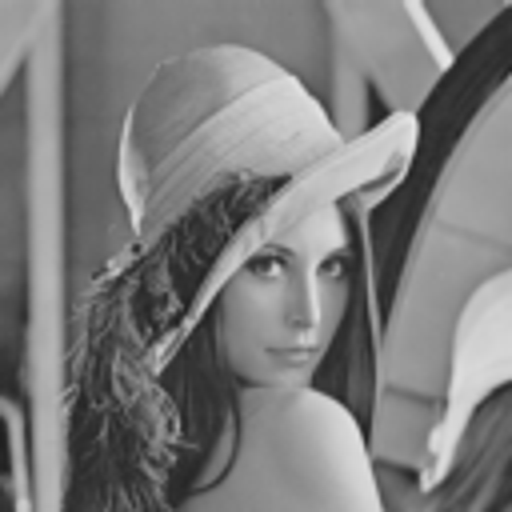
\includegraphics[width=0.45\linewidth]{digitalZoom/lena_BC}
	}
	\caption{Various methods of digitally zooming the Lena test image.}
	\label{fig:digitalZoom.lena}
\end{figure}

\begin{figure}[ht]

\centering
	\subfigure[Original image, PSNR $= \infty$]{
	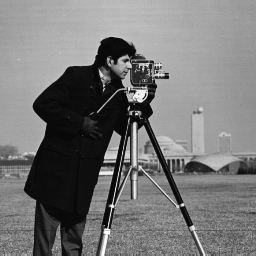
\includegraphics[width=0.45\linewidth]{digitalZoom/cameramanBase}
	}
	\subfigure[Nearest Neighbour, PSNR = +32.91 dB]{
	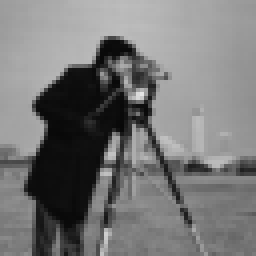
\includegraphics[width=0.45\linewidth]{digitalZoom/cameraman_NN}
	}
	\subfigure[Bilinear Interpolation, PSNR = +32.62 dB]{
	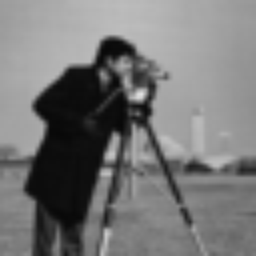
\includegraphics[width=0.45\linewidth]{digitalZoom/cameraman_BL}
	}
	\subfigure[Bicubic Interpolation, PSNR = +32.88 dB]{
	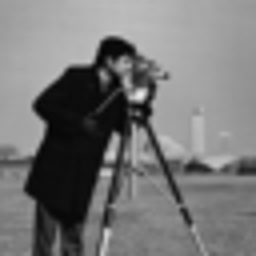
\includegraphics[width=0.45\linewidth]{digitalZoom/cameraman_BC}
	}
	\caption{Various methods of digitally zooming the Cameraman test image.}
	\label{fig:digitalZoom.cameraman}
\end{figure}

Note that since Matlab already has image resizing functions providing the various digital zooming techniques compared, and the lab instructions have not explicitly asked for a implementation, the Matlab function \texttt{imresize} is used.



\subsection{Discussion questions}

\subsubsection{What can you observed about the up-sampled images produced by each of the methods?}

Taking a look at the up-sampled images in Figures~\ref{fig:digitalZoom.lena}~and~\ref{fig:digitalZoom.cameraman} we can qualitatively observe that the images look different.

The \emph{Nearest Neighbour} digital zooming approach has a blocky look (zooming the PDF or viewing a hard-copy is necessary due to the limited PPI of LCD displays). This gives a blocky look to the image, as the algorithm is replacing each 1 pixel in the reduced size image with 16 of the same colour.

The \emph{Bilinear Interpolation} digital zooming approach has a blurred appearance. Bilinear interpolation interpolates using a quadratic polynomial (2 linear lookups); which smooths out the transitions between pixels. In low frequency detail regions, the transition looses the blocky look of the nearest neighbour zooming technique, but in high frequency areas the image loops blurry.

The \emph{Bicubic Interpolation} digital zooming approach has the best subjective appearance. Bicubic interpolation uses 16 pixels in order to derive the polynomial to lookup the new pixel values. Using a higher order polynomial allows detail to be better preserved in high frequency detail areas.

\subsubsection{How do the different methods compare to each other in terms of PSNR as well as visual quality? Why?}

As higher order digital zooming methods are used, the PSNR increases. Information is lost when the image is down-sampled by a factor of 4 using the 1st order image resizing method. The higher order up-sampling methods are better at reconstructing high frequency detail from the down-sampled image and therefore appear less fuzzy than the lower order methods. The higher order methods are also better at preserving edge contrast, which increases the perceived sharpness of the image; therefore the image looks ``better''.

\subsubsection{What parts of the image seems to work well using these digital zooming methods? What parts of the
image doesn't? Why?}

In large solid colour areas, all of the digital zooming methods perform equally. Lena's right shoulder is an area containing low frequency detail that looks very similar among all methods.

Low frequency gradations in the images look better using bilinear and bicubic, as interpolation allows for smooth transition between pixels. This is visible in the shading on Lena's face and the background of the Cameraman photo.

Image edges loose the staircase effect due to interpolation reducing edge aliasing. The edges of the photographer in the Cameraman photo look much better in the bilinear and bicubic photos.


High frequency details, such as Lena's eyes and the feathers in Lena's hat, look better in the bicubic and nearest neighbour digital zooms. The bilinear approach over-smooths the features of the images, and the detail contrast is reduced. The higher order interpolation is able to better interpolate the high frequency data and represent the eyes and feathers accurately.


\subsubsection{Compare the zooming results between Lena and Cameraman. Which image results in higher PSNR? Why?}

The digital zooms of Lena have higher PSNR for all digital zooming methods. This is because the Lena image has less high frequency components than the Cameraman image. Since all interpolation methods work more poorly with the high frequency areas of the image, an image that is composed of more high frequency components will look worse than one with fewer when zoomed using interpolation.


\subsubsection{Which image looks better when restored to the original resolution using digital zooming methods?}

Subjectively (and objectively according the to the PSNR measure), the Lena image looks closer to the original when zoomed using all digital zooming methods.


\subsubsection{What does the PSNR tell you about each of the methods? Does it reflect what is observed visually?}

Since PSNR quantifies the error in the image from the ground truth image, it illustrates that the two images compared using the PSNR measure are similar in intensity at the same points.

The images with higher PSNR generally look subjectively better. The exception is that the nearest neighbour Lena image looks better than bilinear Lena due to the blurriness induce by the bilinear interpolation. There exist other more complicated methods such as the Structural Similarity Method \cite{ssim-image-qual} and the Universal Image Quality Assessment Method \cite{universal-image-qual} (among many others) which may come to the same conclusion that I did about the images, as PSNR does not take into account the psycho-visual model of human vision.


\clearpage
\section{Discrete convolution for image processing}

Discrete convolution takes a kernel and convolves it with the image in question. It can be used to apply various spatial operations to an image, and can also be represented as multiplication in the frequency domain. Seldom is direct convolution performed, as using a fast-Fourier-transform, multiplying and performing a inverse-fast-Fourier-transform is much easier computationally.

\begin{figure}[ht]
\centering
	\subfigure[Original image]{
	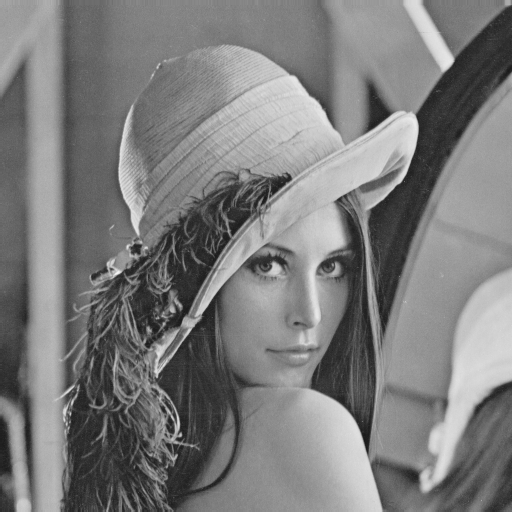
\includegraphics[width=0.45\linewidth]{discreteConvolution/lenaBase}
	}
	\subfigure[(0.16, 0.16, 0.16, 0.16, 0.16, 0.16) kernel]{
	%\caption{Convolved with $\left [ 0.16, 0.16, 0.16, 0.16, 0.16, 0.16\right ]$}
	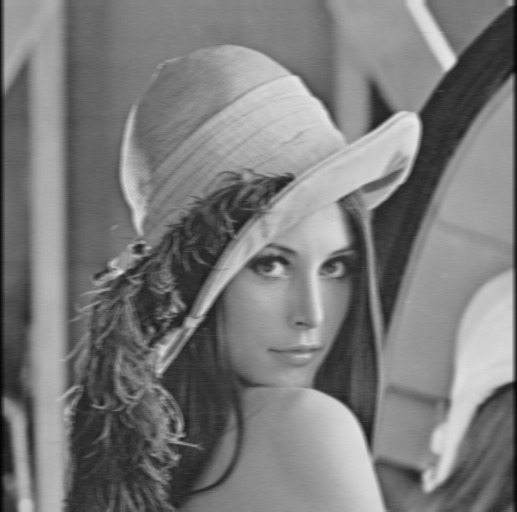
\includegraphics[width=0.45\linewidth]{discreteConvolution/lena_h1}
	}
	\subfigure[(0.16, 0.16, 0.16, 0.16, 0.16, 0.16)$^T$ kernel]{
	%\caption{Convolved with $\left [0.16, 0.16, 0.16, 0.16, 0.16, 0.16\right ]^\textup{T}$}
	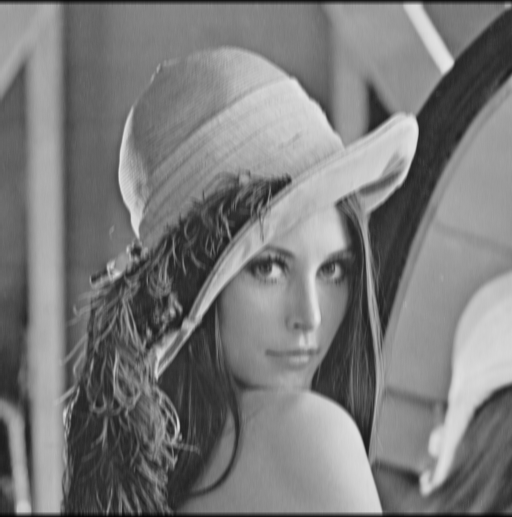
\includegraphics[width=0.45\linewidth]{discreteConvolution/lena_h2}
	}
	\subfigure[(1, -1) kernel]{
	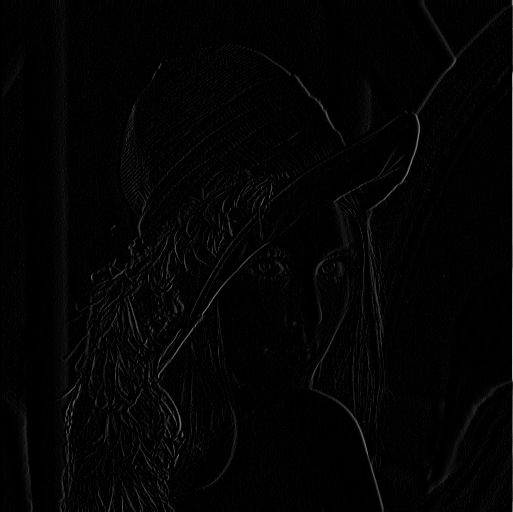
\includegraphics[width=0.45\linewidth]{discreteConvolution/lena_h3}
	}
	\caption{The Lena test image convolved with various kernels.}
	\label{fig:discreteConvolution.lena}
\end{figure}


\subsubsection{What did convolving the image with h1 do to the image? Looking at the impulse function, explain why convolving the image with h1 yields such results.}

Convolving the image with the h1 kernel blurred the image in the horizontal direction (applied a low pass filter in only the horizontal direction). Examining the impulse function, the convolution resulted in a blur in only the horizontal direction as the filter averages the intensity of the image spatially only horizontally. 

\subsubsection{What did convolving the image with h2 do to the image? Looking at the impulse function, explain why convolving the image with h2 yields such results.}

Convolving the image with the h2 kernel blurred the image in the vertical direction (applied a low pass filter in only the vertical direction). Examining the impulse function, the convolution resulted in a blur in only the vertical direction as the filter averages the intensity of the image spatially only vertical. 


\subsubsection{What did convolving the image with h3 do to the image? Looking at the impulse function, explain why convolving the image with h1 yields such results.}

The convolution of the image with h3 resulted in finding the horizontal edge of the image with a first order filter. This filter will respond strongly areas in the image where the image intensity is changing. As the filter is a ``horizontal'' filter, it will respond strongest to horizontal edges, and less so to diagonal edges. The magnitude of the change in intensity will also scale the edge response.

\subsubsection{Based on these results, what role can convolution perform in the context of image processing?}

Convolution can perform operations on an image to extract various spatial components and features of the image. When blurring the image, the convolution was emphasizing the low frequency components of the image, when finding the edges, the convolution was reducing the image to only it's high frequency components.

\clearpage
\section{Fourier analysis}

\begin{figure}[ht]
\centering
	\subfigure[Spectra of rectangle]{
	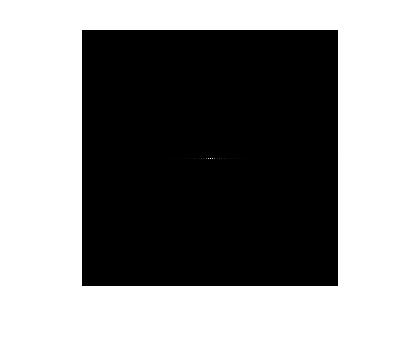
\includegraphics[width=0.45\linewidth]{fourierSpectra/rectangleSpectra}
	}
	\subfigure[Spectra of rotated rectangle]{
	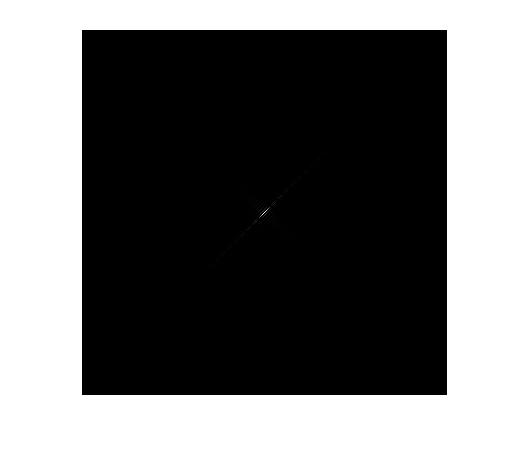
\includegraphics[width=0.45\linewidth]{fourierSpectra/rectangleSpectra45}
	}
	\subfigure[Magnitude Lena Image]{
	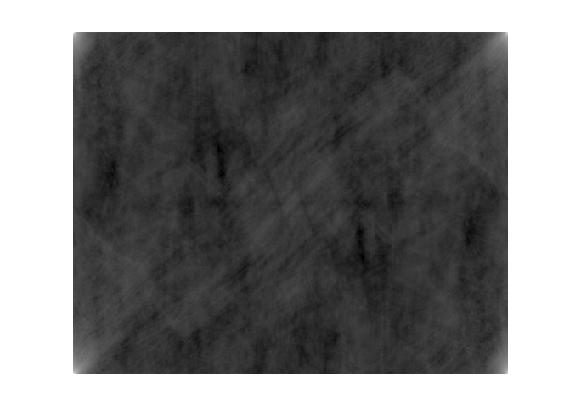
\includegraphics[width=0.45\linewidth]{fourierSpectra/lenamag}
	}
	\subfigure[Phase Lena Image]{
	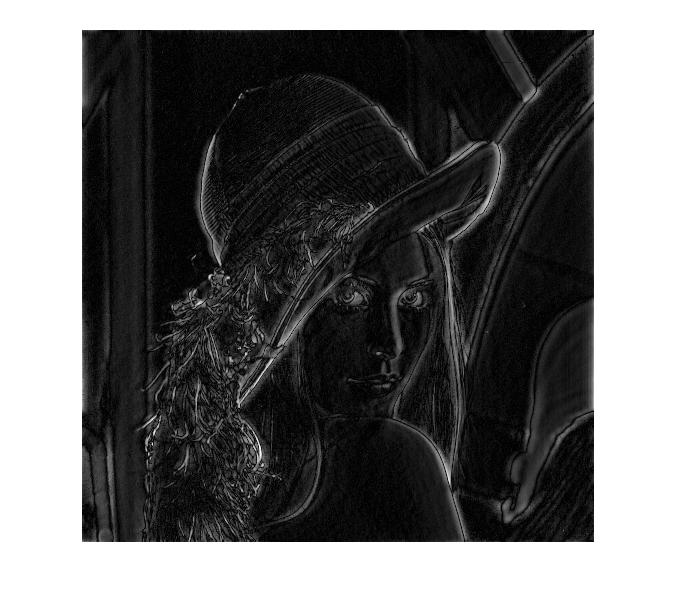
\includegraphics[width=0.45\linewidth]{fourierSpectra/lenaphase}
	}
	\caption{The resulting images for the Fourier Spectra sections}
	\label{fig:fourierSpectra.lena}
\end{figure}


\subsection{Discussion Questions}

\subsubsection{What can you say about the general distribution of energy in the Fourier spectra? Why?}
The distrubution of energy is mostly in the center (i.e. mostly low frequency) in the form of a sinc function. This is because in a plain rectangle, there is mostly course detail.

\subsubsection{ What characteristics about the test image can you infer from the Fourier spectra}
From the spectra, one can infer that the image does not have much in the way of fine details.

\subsubsection{How did the Fourier spectra change from the original image (before rotation)}
The Fourier spectra also rotated 45 degrees.

\subsubsection{ What conclusions and observations can be made about image characteristics based on the Fourier
spectra of both original image and the rotated image}


\subsubsection{Describe how the reconstructed image from the amplitude component look like? What image characteristics does the amplitude component capture}



\subsubsection{Describe how the reconstructed image from the phase component look like? What image characteristics does the phase component capture}
The phase image looks similar to an edge map of the original Lena image. The phase contains the strutural information of the image


\section{Point operations}

Point operations in an image are applied to each point independently of the points in the spatial vicinity.

\subsection{Image histogram}

\begin{figure}[ht]
\centering
	\subfigure[Original image]{
	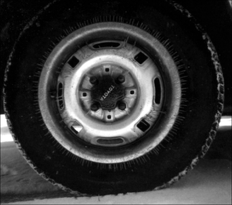
\includegraphics[width=0.45\linewidth]{pointOperations/tireBase}
	}
	\subfigure[Original image histogram]{
	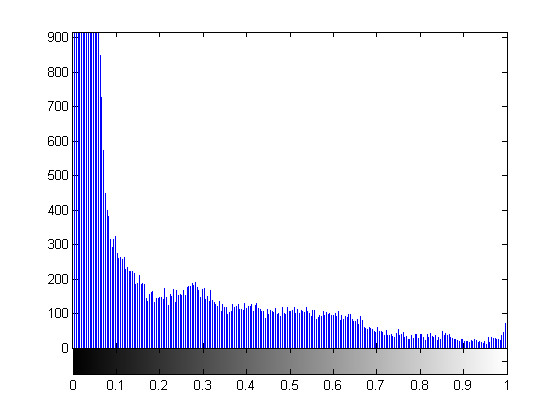
\includegraphics[width=0.45\linewidth]{pointOperations/tireBase_hist}
	}
	\caption{The original image and histogram}
	\label{fig:hist-original}
\end{figure}

\subsubsection{Explain what the histogram of an image represents. Why is it useful?}

A histogram displays the relative distribution of intensities in an image. It is useful for viewing where information in the image is concentrated and can be used to guide rescaling of the image intensities to maximize apparent contrast in the image.

\subsubsection{Describe how the histogram looks like in the context of intensity distribution. What does the histogram say about the image?}

The histogram in Figure~\ref{fig:hist-original} has the majority of it's intensities located in the lower end; black and dark grey dominate the image. The image is a dark image, which have an apparent increase in contrast if grey level expansion is used.

\subsection{Negative image histogram}

\begin{figure}[ht]
\centering
	\subfigure[Negative image]{
	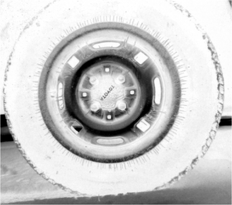
\includegraphics[width=0.45\linewidth]{pointOperations/tireNeg}
	}
	\subfigure[Negative image histogram]{
	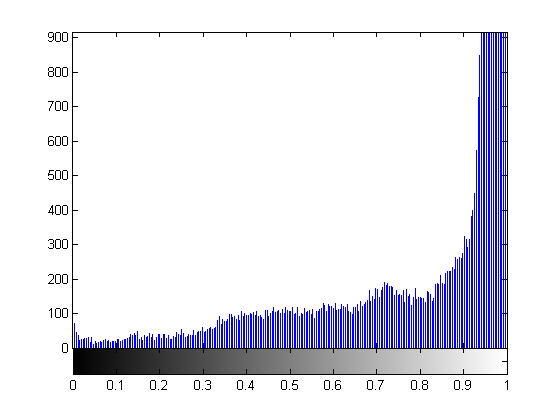
\includegraphics[width=0.45\linewidth]{pointOperations/tireNeg_hist}
	}
	\caption{The negative image and histogram}
	\label{fig:hist-neg}
\end{figure}

\subsubsection{Describe how the histogram looks like in the context of intensity distribution. How does it differ from
the histogram of the original image? Why?}

The histogram in Figure~\label{fig:hist-neg} is a flipped version of the histogram in Figure~\label{fig:hist-original}, unsurprisingly, as the image has been flipped by taking the absolute value of the image subtracting the maximum possible intensity.

In the image and the histogram, white and light grey dominate; and the image may benefit from grey level compression.

\subsection{Power-law transformations}

\begin{figure}[ht]
\centering
	\subfigure[Grey-level expansion with $\gamma = 0.5$]{
	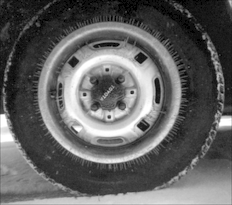
\includegraphics[width=0.45\linewidth]{pointOperations/tire_0_5}
	}
	\subfigure[Grey-level expansion histogram with $\gamma = 0.5$]{
	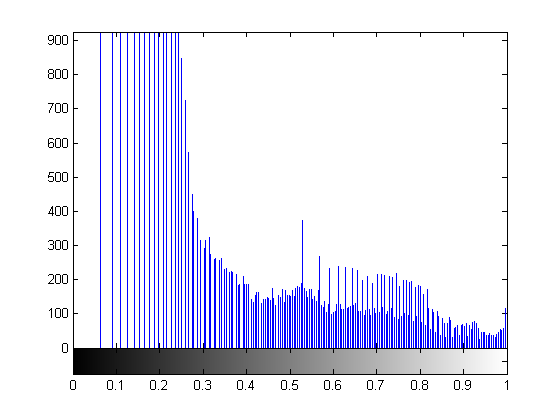
\includegraphics[width=0.45\linewidth]{pointOperations/tire_0_5_hist}
	}
	\subfigure[Grey-level compression with $\gamma = 1.3$]{
	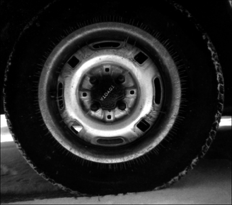
\includegraphics[width=0.45\linewidth]{pointOperations/tire_1_3}
	}
	\subfigure[Grey-level compression histogram with $\gamma = 1.3$]{
	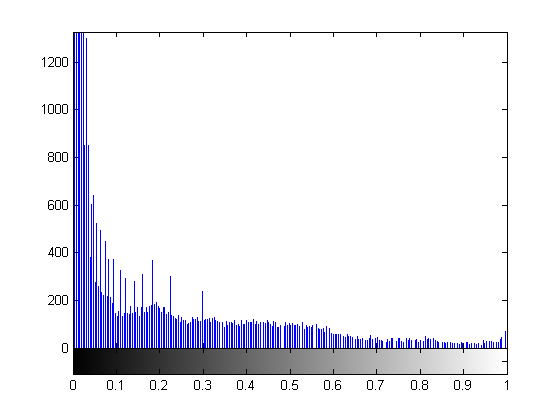
\includegraphics[width=0.45\linewidth]{pointOperations/tire_1_3_hist}
	}
	\caption{Image gamma adjustments and histograms}
	\label{fig:hist-powerlaw}
\end{figure}

\subsubsection{Describe the appearance of the transformed images. Why do they appear this way?}

The image transformed using grey level expansion appears to have more detail on the tire. The grey level expansion expands the dynamic range in the lower half of the intensities of the image, while compressing the dynamic range in the upper half of the intensities of the image.

The image transformed using grey level expansion has less apparent detail. As the majority of the detail in the image was in the lower intensities, and these intensities have been mapped to a lower dynamic range; the contrast between the majority of the intensities in the image has been reduced. However, more detail can be seen in the snow underneath the tire, as it's dynamic range has been expanded.

\subsubsection{Describe how each of the histogram looks like in the context of intensity distribution. Why do they look like this? What does each histogram say about each transformed image?}

The grey-level expansion histogram has the low intensity image detail from the original image spread out over a greater dynamic range. This image has better contrast as the intensities in the image are well distributed.

The grey level compression histogram has the low intensity image detail from the original image mapped to a smaller dynamic range. Observing the histogram, most of the detail in the image is constricted between (0, 0.03), which can be observed in the image, with most of the details imperceptible from the low frequency components.

\subsubsection{Compared with the original image, which of the transforms should you use to enhance the image? Why?}

I would use the grey-level expansion to enhance the image. The grey-level expansion makes better use of the dynamic range of the image by spreading out the details in the lower intensities over a greater range of values, increasing the apparent local contrast in the image.

\subsection{Histogram equalization}


\begin{figure}[ht]
\centering
	\subfigure[Histogram equalized image]{
	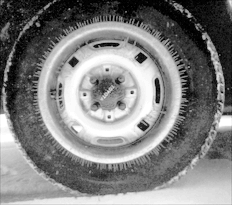
\includegraphics[width=0.45\linewidth]{pointOperations/tire_eq}
	}
	\subfigure[Histogram equalized image histogram]{
	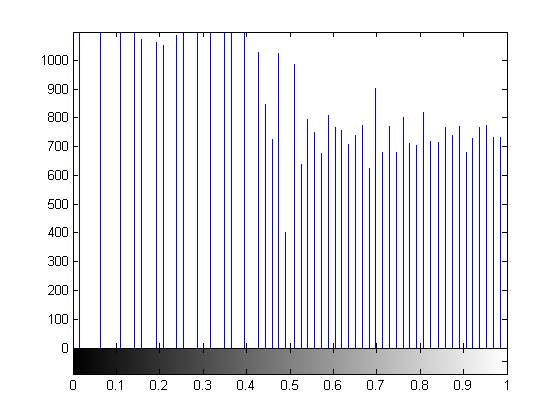
\includegraphics[width=0.45\linewidth]{pointOperations/tire_eq_hist}
	}
\end{figure}

\subsubsection{Describe the appearance of the equalized image}

As the equalized image has a uniform distribution of image intensity values, the image appears to have high local contrast across the whole image. However, the original intensities in the image have not been preserved; the tire is not almost the same shade as the snow.

\subsubsection{Describe how the histogram looks like in the context of intensity distribution. Why does it look like this? What does each histogram say about each equalized image?}

The histogram has a uniform distribution of intensities. Histogram equalization can be visualized as applying many small power law transformations to the image, each one only applying to a small range of values, until the distribution of intensities is uniform. 

The histogram demonstrates that the intensities in the image are uniformly distributed, therefore the average colour in the image is a 50\% grey. The image also will have an equal proportion of each possible intensity of colour.

\appendix
\newpage

\section{Matlab Code}
\subsection{PSNR}
\label{code-PSNR}
\lstinputlisting[language=Matlab]{"matlabFiles/PSNR.m"}


% -------- Bibliography --------
%\addcontentsline{toc}{chapter}{\hspace{13pt} References}
\bibliography{refs}

\end{document}  